\subsection{Application Server}\label{sec:impl-as}

% TODO: Update if something changes
As we previously said in Section \ref{sec:sol-des-as}, our Phoenix Application
Server is composed of two sub-applications, namely \texttt{Domain} and
\texttt{Interface}.

\subsubsection{Domain}

\texttt{Domain} can be roughly seen as a supervision tree, which at the top has
the root \texttt{Domain} module itself. This module supervises $O(k * m)$
modules, where $k$ is the number of cities and $m$ the number of districts per
city.

In Figure \ref{fig:impl-as-domain} we can see a visual representation of this
tree: even if in the picture \texttt{DistrictInfo} GenServers (i.e., the
per-district trackers) are grouped by city (e.g., $A$ in the drawing), the
supervision tree has an actual depth of 1\footnote{that's why there is a
dotted line around each \texttt{DistrictInfo}}.
We could also have placed one intermediate supervisors for each city, but
there was no special need to do it.

Always in Figure \ref{fig:impl-as-domain}, we can notice that there is another
GenServer supervised other than the \texttt{DistrictInfo}s: this is the
\texttt{Loader} module, which is responsible for loading static information in
the district trackers when our Application Server starts. We chose to employ a
supervised GenServer (that can be also viewed as an Elixir process) and not a
task because we use the \texttt{Loader} module at runtime too, when a
simulation ends and we want to reset a district tracker to its initial
configuration values.

\begin{figure}[H]
  \centering
  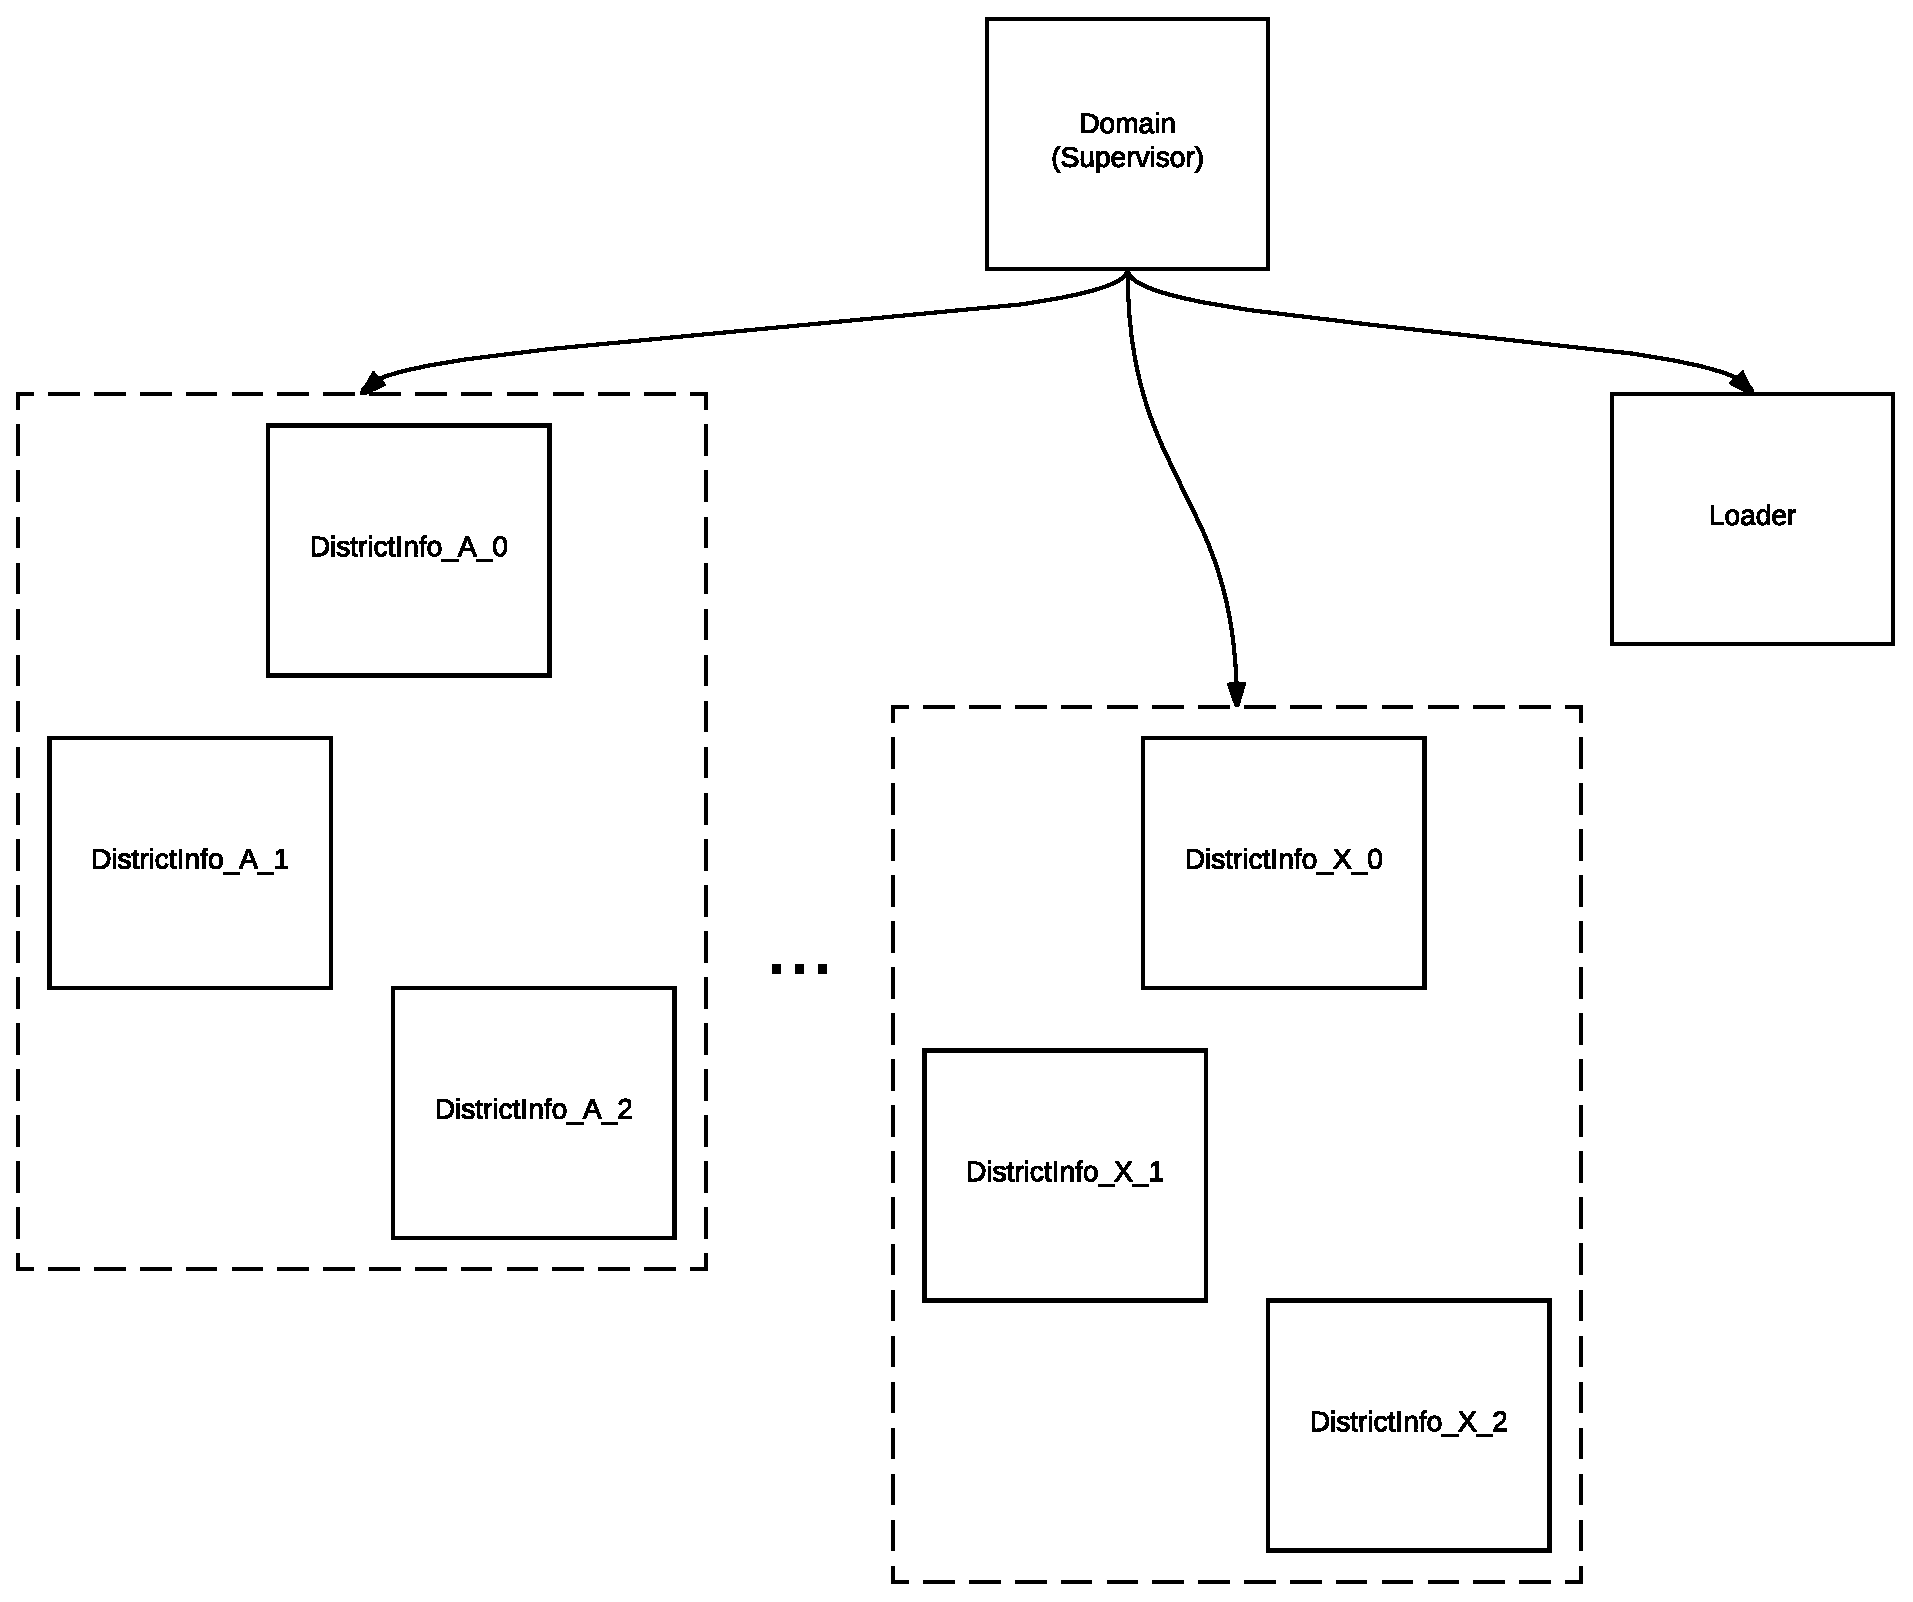
\includegraphics[width=\columnwidth]{images/implementation/as-domain.eps}
  \caption{Domain supervision tree}
  \label{fig:impl-as-domain}
\end{figure}

\subsubsection{Interface}

Even if we implemented several modules and REST APIs, we will focus on some
key components of the \texttt{Interface} sub-system.

\paragraph{PubSub}
We'll start by talking about \texttt{DistrictChannel}, which is an
implementation we provided for the \texttt{Channel} behaviour. As we can see
in Figure \ref{fig:impl-as-pubsub}, we subscribe \texttt{UserSocket}s to the
Phoenix pub/sub system for the city simulator.
Sockets reach \texttt{DistrictChannel} through an \texttt{Endpoint}.
Each socket is always subscribed to a district, and could be additionally
subscribed to a traveller. Therefore:

\begin{itemize}
  \item when a user requires to join the \texttt{DistrictChannel}, it will
    be immediately subscribed to the district she is interested in;
  \item later on, the user may request to have updates on a specific traveller
    by making a subscription to a specific traveller topic.
\end{itemize}

Finally, in \texttt{DistrictChannel} we filter (and eventually process)
outgoing information by implementing specific \texttt{handle\_out} callbacks.
Thanks to this, we are able to avoid unnecessary traffic towards the clients.

\paragraph{Input pipeline}
Events and updates arrive at the application server starting from an
\texttt{InputStream}. This process is a Wabbit GenStage produces which
basically receives messages from a RabbitMQ topic exchange and forwards them
to a \texttt{Formatter}.
A \texttt{Formatter} is a process which just extracts basic information from
the incoming messages and transform them in a format used by the application
server processes.
Then messages are piped through an \texttt{InternalDispatcher} process, which
can eventually dispatch some information to some processes in the Application
Server; for example, it sends updates to district trackers when a traveller
moves from a district to another one.
Finally, messages are broadcasted to the Interface \texttt{Endpoint} by
providing the payload and the topic of a message.

\paragraph{Output}

\begin{figure}[H]
  \centering
  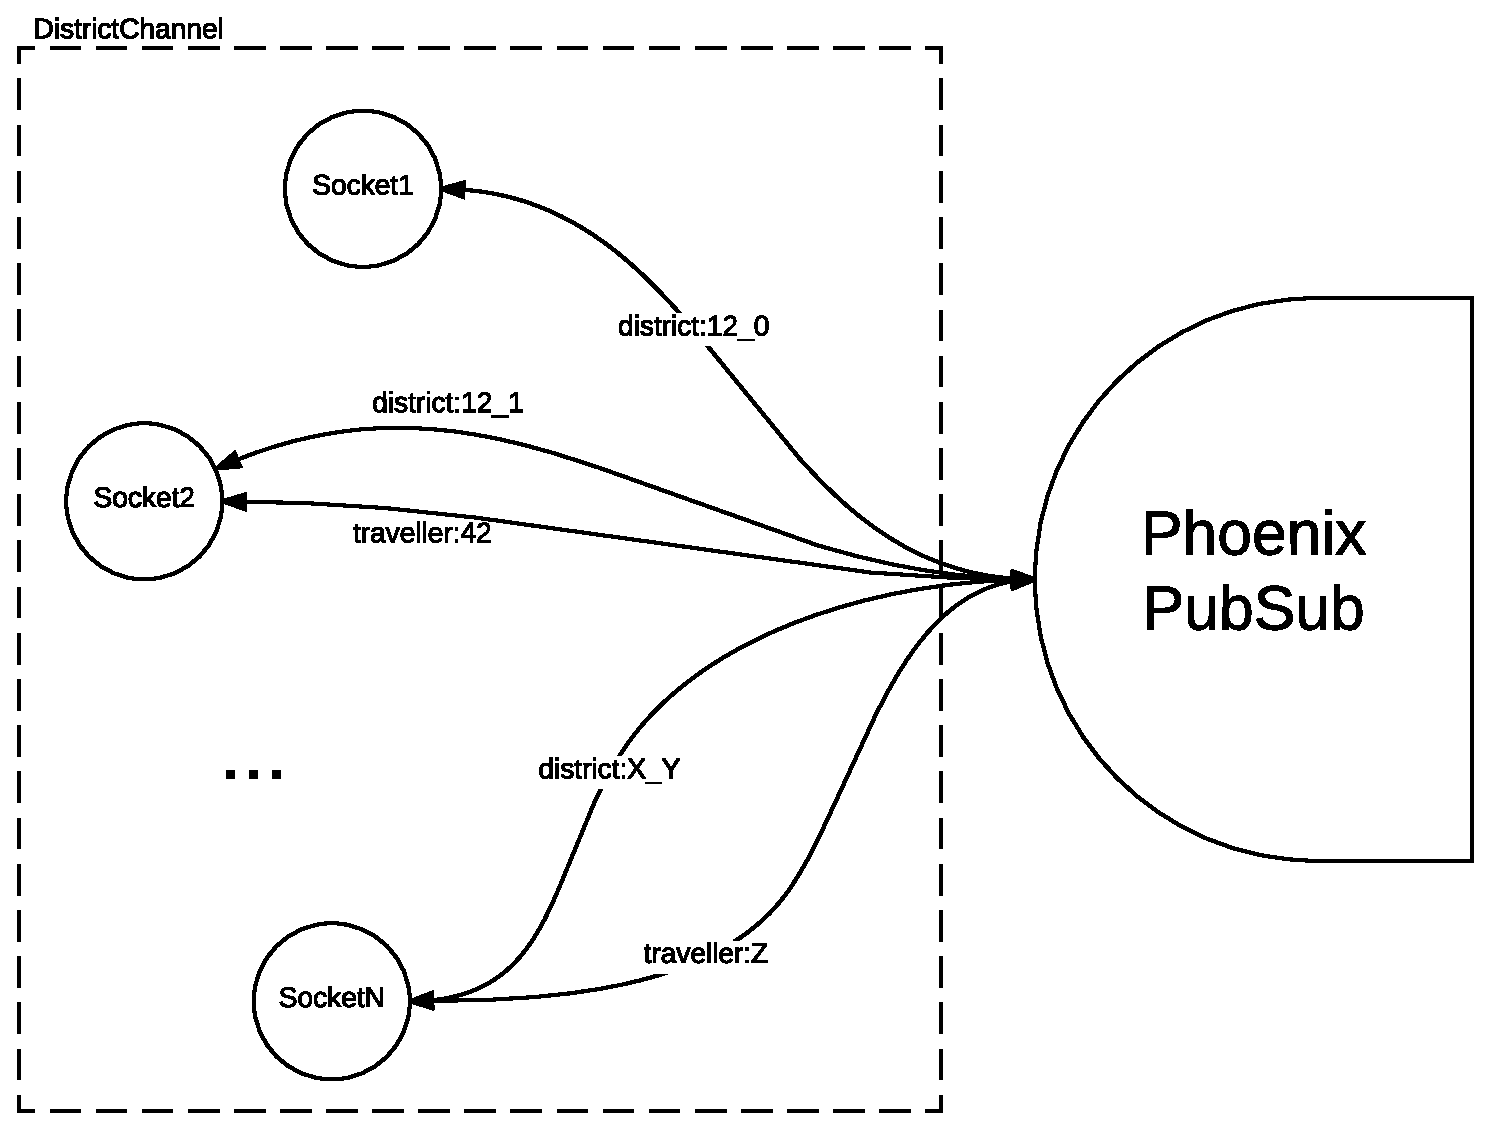
\includegraphics[width=1.1\columnwidth]{images/implementation/as-chan-pubsub.eps}
  \caption{Application Server architecture}
  \label{fig:impl-as-pubsub}
\end{figure}
